\documentclass[xetex]{scrartcl}

% packages
\usepackage{xltxtra}
\usepackage{polyglossia}
\usepackage[
    urlcolor=black,
    linkcolor=black,
    citecolor=black,
    filecolor=black,
    pagecolor=black,
    linktocpage=true,
    ]{hyperref}
\usepackage{fontspec}
\usepackage{scrpage2}
\usepackage[left=2cm,right=2cm,top=3cm,bottom=3cm]{geometry}
\usepackage{colortbl}
\usepackage{alltt}
\usepackage{listings}
\usepackage{multirow}

% fonts general
\setmainfont[Mapping=tex-text,Scale=1.0]{FreeSans}
\setsansfont[Mapping=tex-text,Scale=1.0]{FreeSans}
\setmonofont{FreeMono}

% special fonts
\newfontfamily\hana{HAN NOM A}
\newfontfamily\hanb{HAN NOM B}
\newfontfamily\sil{Charis SIL}





\newcommand{\White}[1]{\cellcolor{white} \textcolor{black}{ #1}}

% language settings
\setmainlanguage{english}
\setotherlanguage{german}

% pagestyle settings
\pagestyle{scrheadings}
\ihead{M.-S. Wu and J.-M. List}
\chead{Computer-Assisted Language Comparison}
\ohead{+++DATE+++}
\ifoot{}
\cfoot{\pagemark}
\ofoot{}

\usepackage[
    alldates=terse,
    backend=bibtex,
    %backref=true,
    bibstyle=authoryear,
    firstinits=true,
    ibidtracker=strict,
    isbn=false,doi=false,url=false,
    labelnumber=true,
    loccittracker=strict,
    hyperref=false,
    maxbibnames=10,
    maxcitenames=2,
    natbib=true,
    opcittracker=strict,
    sortcites=true,
    sorting=nyt,
    defernumbers=true,
    style=authoryear-ibid,
    terseinits=false
    ]{biblatex}

% Diese Datei beinhaltet alle Angaben für die Bibliographieeinstellungen. Dabei
% werden die Vorgaben des authoryear-Styles von biblatex verändert.

%%%%%%%%%%%%%%%%%%%%%%%%%%%%%%%%%%%%%%%%%%%%%%
% Sprachstrings für Übersetzungen definieren %
%%%%%%%%%%%%%%%%%%%%%%%%%%%%%%%%%%%%%%%%%%%%%%
% translator origlanguage strings
\NewBibliographyString{fromrussian}
\NewBibliographyString{fromchinese}
\NewBibliographyString{fromfrench}
\NewBibliographyString{fromserbocroatian}
\NewBibliographyString{fromgreek}
\NewBibliographyString{fromenglish}
\NewBibliographyString{fromquiche}
\NewBibliographyString{fromsanskrit}

% special editorrole-strings
\NewBibliographyString{bygreektext}
\NewBibliographyString{bygermantext}
\NewBibliographyString{byfrenchtext}
\NewBibliographyString{byenglishtext}
\NewBibliographyString{byrussiantext}
\NewBibliographyString{bylatintext}
\NewBibliographyString{byrectrans}
\NewBibliographyString{bytechnical}
\NewBibliographyString{bydesigncoding}

% specific stuff
\NewBibliographyString{specialenglishtranslation}
\NewBibliographyString{specialgermantranslation} 
\NewBibliographyString{specialoriginaledition} 
\NewBibliographyString{specialcriticaledition}
\NewBibliographyString{specialgermanedition}
\NewBibliographyString{specialenglishedition}
\NewBibliographyString{specialelectronicedition}
\NewBibliographyString{specialbc}
\NewBibliographyString{specialbetween}
\NewBibliographyString{specialca}
\NewBibliographyString{specialad}
\NewBibliographyString{specialbefore}
\NewBibliographyString{specialafter}
\NewBibliographyString{reissue}
\NewBibliographyString{procsym}
\NewBibliographyString{paperworkshop}
\NewBibliographyString{paperconference}
\NewBibliographyString{talkatm}
\NewBibliographyString{talkatf}

\DefineBibliographyStrings{english}{%
% translator-strings origlanguage
fromrussian={from the Russian},
fromchinese={from the Chinese},
fromfrench={from the French},
fromserbocroatian={from the Serbo-Croatian},
fromgreek={from the Greek},
fromenglish={from the English},
fromgerman={from the German},
fromquiche={from the Quiche},
fromsanskrit={from the Sanskrit},
% editor-strings special type
bygreektext={Greek text by},
bygreektext={Greek text by},
byenglishtext={English text by},
bygermantext={German text by},
byrussiantext={Russian text by},
byfrenchtext={French text by},
bylatintext={Latin text by},
bytechnical={Technical implementation by},
byrectrans={Recordings and transcriptons by},
bydesigncoding={Page design and coding by},
% special types
specialenglishtranslation={English translation},
specialgermantranslation={German translation},
specialoriginaledition={Original edition},
specialcriticaledition={Critical edition},
specialelectronicedition={Electronic Edition},
specialbc={BC},
specialad={AD},
specialca={ca.},
specialbetween={between}
specialbefore={before},
specialafter={after},
specialgermanedition={German edition},
specialenglishedition={English edition},
reissue = {Reissue},
procsym={Proceedings of the Symposium},
paperworkshop={Paper, presented at the workshop},
paperconference={Paper, presented at the conference},
talkatm={Talk, held at the},
talkatf={Talk, held at the}
}

\DefineBibliographyStrings{german}{%
% origlanguage
fromenglish={a. d. Englischen},
fromrussian={a. d. Russischen},
fromchinese={a. d. Chinesischen},
fromfrench={a. d. Französischen},
fromserbocroatian={a. d. Serbokroatischen}
fromgreek={a. d. Griechischen},
fromenglish={a. d. Englischen},
fromgerman={a. d. Deutschen},
fromquiche={a. d. Quiche},
fromsanskrit={a. d. Sanskrit},
% editor-roles
bygreektext={Griechischer Text von},
byenglishtext={Englischer Text von},
bygermantext={Deutscher Text von},
byrussiantext={Russischer Text von},
byfrenchtext={Französischer Text von},
bylatintext={Lateinischer Text von},
bytechnical={Technische Implementierung von},
byrectrans={Aufnahmen und Transkriptionen von},
bydesigncoding={Webdesign und Programmierung von},
% tests
specialenglishtranslation={Englische Übersetzung},
specialgermantranslation={Deutsche Übersetzung},
specialoriginaledition={Ursprüngliche Ausgabe},
specialcriticaledition={Kritische Edition},
specialelectronicedition={Elektronische Edition},
specialbc={v. Chr.},
specialad={n. Chr.},
specialca={ca.},
specialbetween={zwischen},
specialbefore={vor},
specialafter={nach},
specialgermanedition={Deutsche Ausgabe},
specialenglishedition={Englische Ausgabe},
reissue={Neuaufl.},
procsym={Tagungsbericht der Tagung},
paperworkshop={Vortrag, gehalten auf dem Workshop},
paperconference={Vortrag, gehalten auf der Konferenz},
talkatm={Vortrag, gehalten am},
talkatf={Vortrag, gehalten an der}
}

%%%%%%%%%%%%%%%%%%%%%%%%%%%%%%%%%%%%%%%%%%%%%%%%%
% Übersetzungen und Originalschriften von Titel %
%%%%%%%%%%%%%%%%%%%%%%%%%%%%%%%%%%%%%%%%%%%%%%%%%
\renewbibmacro*{title}{%
  \ifboolexpr{
    test {\iffieldundef{title}}
    and
    test {\iffieldundef{subtitle}}
  }
    {}
    {\printtext[title]{%
\printfield[titlecase]{title}%
\iffieldundef{subtitle}{}{\setunit{\subtitlepunct} \printfield[titlecase]{subtitle}}%
\iffieldundef{userb}{}{{\addspace{\normalfont\printfield{userb}}}}%
\iffieldundef{usera}{}{\addspace\textit{\em [\printfield{usera}]}}}%
\newunit}%
\printfield{titleaddon}}

%%%%%%%%%%%%%%%%%%%%%%%%%%%%%%%%%%%%%%%%%%%%%%%%%
% Übersetzungen und Originalschriften von Titel %
%%%%%%%%%%%%%%%%%%%%%%%%%%%%%%%%%%%%%%%%%%%%%%%%%
\renewbibmacro*{booktitle}{%
\ifboolexpr{
  test {\iffieldundef{booktitle}}
  and
  test {\iffieldundef{booksubtitle}}
}
  {}
  {\printtext[booktitle]{%
     \printfield[titlecase]{booktitle}%
     \iffieldundef{booksubtitle}{}{\setunit{\subtitlepunct}%
     \printfield[titlecase]{booksubtitle}}%
     \iffieldundef{userd}{}{{\addspace\textnormal{\printfield{userd}}}}%
\iffieldundef{userc}{}{\addspace\textit{\em [\printfield{userc}]}}}
   \newunit}%
\printfield{booktitleaddon}}

%%%%%%%%%%%%%%%%%%%%%%%%%%%%%%%%%%%%%%%%%%%%%%%%%
% Übersetzungen und Originalschriften von Titel %
%%%%%%%%%%%%%%%%%%%%%%%%%%%%%%%%%%%%%%%%%%%%%%%%%
\renewbibmacro*{maintitle}{%
  \ifboolexpr{
    test {\iffieldundef{maintitle}}
    and
    test {\iffieldundef{mainsubtitle}}
  }
    {}
    {\printtext[maintitle]{%
       \printfield[titlecase]{maintitle}%
       \iffieldundef{mainsubtitle}{}{\setunit{\subtitlepunct}%
       \printfield[titlecase]{mainsubtitle}}%
\iffieldundef{verbb}{}{{\addspace\printfield{verbb}}}%
\iffieldundef{verba}{}{\addspace\textit{\em [\printfield{verba}]}}}
   \newunit}%
  \printfield{maintitleaddon}}

%%%%%%%%%%%%%%%%%%%%%%%%%%%%%%%%%%%%%%%%%%%%%%%%%%%%%%
% Neue Makros für komplexe Datenangaben von Reprints %
%%%%%%%%%%%%%%%%%%%%%%%%%%%%%%%%%%%%%%%%%%%%%%%%%%%%%%

%%%%%%%%%%%%%%%%%%%%%%%%%%%%%%%
% Neues Bibmakro für Pubstate %
%%%%%%%%%%%%%%%%%%%%%%%%%%%%%%%
\newbibmacro*{pubstate}{%
{\iffieldundef{pubstate}}
{}
{\printfield{pubstate}}}

%%%%%%%%%%%%%%%%%%%%%%%%%%%%%%%%
% Neues macro für howpublished %
%%%%%%%%%%%%%%%%%%%%%%%%%%%%%%%%
\newbibmacro*{howpublished}{%
\iffieldundef{howpublished}
{}
{\ifbibxstring{\thefield{howpublished}}
{\bibstring{\thefield{howpublished}}}
{\printtext{\thefield{howpublished}}}}}

%%%%%%%%%%%%%%%%%%%%%%%%%%%%%%%%%%%%%%%%%%%%%%%%%%%
% Füge origdate in die entsprechenden Makros ein  %
%%%%%%%%%%%%%%%%%%%%%%%%%%%%%%%%%%%%%%%%%%%%%%%%%%%
%\renewbibmacro*{cite}{%
%\iffieldundef{shorthand}
%{\ifthenelse{\ifnameundef{labelname}\OR
%\iffieldundef{year}}
%{\usebibmacro{cite:label}}
%{\printtext[bibhyperref]{\printnames{labelname}}%
%\nameyeardelim
%\usebibmacro{cite:labelyear+extrayear}}}
%{\usebibmacro{cite:shorthand}}}
%\renewbibmacro*{cite}{%
%\iffieldundef{shorthand}
%{\ifthenelse{\ifnameundef{labelname}\OR
%\iffieldundef{year}}
%{\usebibmacro{cite:label}}
%{\printtext{\printnames{labelname}}%
%\nameyeardelim
%\usebibmacro{cite:labelyear+extrayear}}}
%{\usebibmacro{cite:shorthand}}}
%
%
%
%\renewbibmacro*{textcite}{%
%\ifnameundef{labelname}
%{\iffieldundef{shorthand}
%{\usebibmacro{cite:labelyear+extrayear}}
%{\usebibmacro{cite:shorthand}}}
%{\printtext{\printnames{labelname}}%
%\addspace\bibleftparen
%\iffieldundef{shorthand}
%{\iffieldundef{year}
%{\usebibmacro{cite:label}}
%{\usebibmacro{cite:labelyear+extrayear}}}
%{\usebibmacro{cite:shorthand}}}}
%
\renewbibmacro*{cite:shorthand}{%
  \printtext{\printfield{shorthand}}}

\renewbibmacro*{cite:labeldate+extradate}{%
\iffieldundef{labelyear}
{}
{\printtext[bibhyperref]{%
\iffieldundef{origyear}
{\printfield{labelyear}}
{\printfield{origyear} [\printfield{labelyear}]}%   <--- added
%[\printfield{labelyear}]%
%\printfield{extrayear}
}}}

%%%%%%%%%%%%%%%%%%%%%%%%%%%%%%%%%%%%%
% Origdate und Date: 1950 [1995] an.%
%%%%%%%%%%%%%%%%%%%%%%%%%%%%%%%%%%%%%
\renewbibmacro*{date+extradate}{%
\iffieldundef{year}
{}
{\printtext[parens]{%
\iffieldundef{origdate}
{\printdateextra}
{\printfield{origdate} [\printdateextra]}%  <--- added
}}}

%%%%%%%%%%%%%%%%%%%%%%%%%%%%%%%%%%%%%%%%%%%%%%
% origlocation and origpublisher in addendum %
%%%%%%%%%%%%%%%%%%%%%%%%%%%%%%%%%%%%%%%%%%%%%%
% define a bibmacro edition
\newbibmacro*{edition}
{\ifinteger{\thefield{edition}}
{}
{\ifbibxstring{\thefield{edition}}
{\bibstring{\thefield{edition}}}
{\printtext{\thefield{edition}\isdot}}}}

% redefine field format of edition in order to incorporate more information
\DeclareFieldFormat{edition}{%
  \ifinteger{#1}
    {\mkbibordedition{#1}~\bibstring{edition}}
    {\usebibmacro{edition}}}

% reprintorigyearmacro
\newbibmacro*{reprintorigyear}
{\iffieldundef{origyear}
{}
{\printtext{, \printfield{origyear}}}}

% reprintaddendummacro
\newbibmacro*{reprintaddendum}
{\iffieldundef{verbc}
{}
{\printtext{[\usebibmacro{specialedition}:%
\iflistundef{origlocation}
{\iflistundef{origpublisher}
{}
{\addspace\printfield{origpublisher}}}
{\addspace\printlist{origlocation}%
\iflistundef{origpublisher}
{}
{:\addspace\printtext{\printlist{origpublisher}}}%
\iffieldundef{origyear}
{}
{\usebibmacro{reprintorigyear}}}%
]}}}

\renewbibmacro*{addendum+pubstate}{%
\iffieldundef{addendum}
{%
\iffieldequalstr{edition}{reprint}
{\usebibmacro{reprintaddendum}}
}
{\printfield{addendum}}}

%%%%%%%%%%%%%%%%%%%%%%%%%%%
% Characterize Originaleditions %
%%%%%%%%%%%%%%%%%%%%%%%%%%%
\newbibmacro*{specialedition}{%
  \iffieldundef{verbc}
    {}
    {\ifbibxstring{special\thefield{verbc}}
       {\bibstring{special\thefield{verbc}}}
       {\printtext{\thefield{usere}}}}}

\DeclareBibliographyDriver{set}{%
  \entryset{%
\iffieldundef{verbc}
{}
{\usebibmacro{verbc}: }}{}%
  \newunit\newblock
  \usebibmacro{setpageref}%
  \finentry}

%%%%%%%%%%%%%%%%%%%%%%%%%%%
% Characterize Entry Sets %
%%%%%%%%%%%%%%%%%%%%%%%%%%%
\newbibmacro*{special}{%
  \iffieldundef{usere}
    {}
    {\ifbibxstring{special\thefield{usere}}
       {\bibstring{special\thefield{usere}}}
       {\printtext{\thefield{usere}}}}}

\DeclareBibliographyDriver{set}{%
  \entryset{%
\iffieldundef{usere}
{}
{\usebibmacro{special}: }}{}%
  \newunit\newblock
  \usebibmacro{setpageref}%
  \finentry}

%%%%%%%%%%%%%%%%%%%%%%%%%%%%%%%%%%%%%
% commands for citation in the text %
%%%%%%%%%%%%%%%%%%%%%%%%%%%%%%%%%%%%%
\renewcommand{\nameyeardelim}{ }
\renewcommand{\multicitedelim}{, }
\renewcommand{\postnotedelim}{: }
\DeclareFieldFormat{postnote}{#1}
\DeclareFieldFormat{pages}{#1}

%%%%%%%%%%%%%%%%%%%
% Eprint Archives %
%%%%%%%%%%%%%%%%%%%
\DeclareFieldFormat{eprint:gallica}{%
  Gallica\addcolon\space
  \ifhyperref
    {\href{http://gallica.bnf.fr/#1}{\nolinkurl{#1}}}
    {\nolinkurl{#1}}}
\DeclareFieldAlias{eprint:Gallica}{eprint:gallica}

\DeclareFieldFormat{eprint:ia}{%
  Internet Archive \addcolon\space
  \ifhyperref
  {\href{http://www.archive.org/details/#1}{\nolinkurl{#1}}}
  {\nolinkurl{#1}}}
\DeclareFieldAlias{eprint:IA}{eprint:ia}

\DeclareFieldFormat{eprint:gutenberg}{%
  Projekt Gutenberg-DE \addcolon\space
  \ifhyperref
  {\href{http://gutenberg.spiegel.de/buch/#1}{\nolinkurl{#1}}}
  {\nolinkurl{#1}}}
\DeclareFieldAlias{eprint:Gutenberg}{eprint:gutenberg}

\DeclareFieldFormat{eprint:zvdd}{%
 ZVDD \addcolon\space
 \ifhyperref
 {\href{http://www.zvdd.de/dms/load/met/?PPN=#1}{\nolinkurl{#1}}}
 {\nolinkurl{#1}}}
%%%%%%%%%%%%%%%%%%%%%%%%%%%%%%%%%%%%%%%%%%%%%%%%%%%%%%%%%%%%%%%%%%%%%%%%%%%%%%%
% Dieses Makro muss verändert werden, damit bei der Zitation von Sammelwerken %
% der Booktitle als normaler Titel erscheint.                                 %
%%%%%%%%%%%%%%%%%%%%%%%%%%%%%%%%%%%%%%%%%%%%%%%%%%%%%%%%%%%%%%%%%%%%%%%%%%%%%%%
%\renewbibmacro*{maintitle+title}{%
%  \iffieldsequal{maintitle}{title}
%    {\clearfield{maintitle}%
%     \clearfield{mainsubtitle}%
%     \clearfield{maintitleaddon}}
%    {\iffieldundef{maintitle}
%    {\usebibmacro{booktitle}}
%       {\usebibmacro{maintitle}%
%	\newunit\newblock
%	\iffieldundef{volume}
%	  {}
%	  {\printfield{volume}%
%           \printfield{part}%
%           \setunit{\addcolon\space}}}}%
%  \usebibmacro{title}%
%  \newunit}

%%%%%%%%%%%%%%%%%%%%%%%%%%%%%%%%%%
% Erneuere das event-venue-macro %
%%%%%%%%%%%%%%%%%%%%%%%%%%%%%%%%%%
\renewbibmacro*{event+venue+date}{%
\iffieldundef{howpublished}
{%
\iffieldundef{eventtitle}
{%
\ifboolexpr{
    test {\iffieldundef{venue}}
    and
    test {\iffieldundef{eventyear}}
  }
    {}
    {\setunit*{\addspace}%
     \printtext[parens]{%
       \printfield{venue}%
       \setunit*{\addcomma\space}%
       \printeventdate}}%
}
{\printtext{``\printfield{eventtitle}"}%
  \ifboolexpr{
    test {\iffieldundef{venue}}
    and
    test {\iffieldundef{eventyear}}
  }
    {}
    {\setunit*{\addspace}%
     \printtext[parens]{%
       \printfield{venue}%
       \setunit*{\addcomma\space}%
       \printeventdate}}%
       \newunit}}
{\printtext{\usebibmacro{howpublished} }%
\iffieldundef{eventtitle}
{}%
%\ifboolexpr{
%    test {\iffieldundef{venue}}
%    and
%    test {\iffieldundef{eventyear}}
%  }
%    {}
%    {\setunit*{\addspace}%
%     \printtext[parens]{%
%       \printfield{venue}%
%       \setunit*{\addcomma\space}%
%       \printeventdate}}%
%}
{\printtext{``\printfield{eventtitle}"}}%
  \ifboolexpr{
    test {\iffieldundef{venue}}
    and
    test {\iffieldundef{eventyear}}
  }
    {}
    {\setunit*{\addspace}%
     \printtext[parens]{%
       \printfield{venue}%
       \setunit*{\addcomma\space}%
       \printeventdate}}%
       \newunit}}

%%%%%%%%%%%%%%%%%%%%%%%%%%%%%%%%%%%%%%%%%%%%%%%%%%%
% Erstelle einen Driver für talks auf Konferenzen %
%%%%%%%%%%%%%%%%%%%%%%%%%%%%%%%%%%%%%%%%%%%%%%%%%%%
\DeclareBibliographyDriver{customa}{%
  \usebibmacro{bibindex}%
  \usebibmacro{begentry}%
  \usebibmacro{author}%
  \setunit{\labelnamepunct}\newblock
  \usebibmacro{title}%
  \newunit
  \printlist{language}%
  \newunit\newblock
  \usebibmacro{byauthor}%
  \newunit\newblock
  \usebibmacro{event+venue+date}%
  \newunit\newblock
  \printfield{note}%
  \newunit\newblock
  \usebibmacro{location+date}%
  \newunit\newblock
  \iftoggle{bbx:url}
    {\usebibmacro{doi+eprint+url}}
    {}%
  \newunit\newblock
  \usebibmacro{addendum+pubstate}%
  \setunit{\bibpagerefpunct}\newblock
  \usebibmacro{pageref}%
  \usebibmacro{finentry}}

%%%%%%%%%%%%%%%%%%%%%%%%%%%%%%%%%%%%%%%%%
% Neues Makro für Artikel ohne "IN:"    %
%%%%%%%%%%%%%%%%%%%%%%%%%%%%%%%%%%%%%%%%%

\DeclareBibliographyDriver{article}{%
  \usebibmacro{bibindex}%
  \usebibmacro{begentry}%
  \usebibmacro{author/translator+others}%
  \setunit{\labelnamepunct}\newblock
  \usebibmacro{title}%
  \newunit
  \printlist{language}%
  \newunit\newblock
  \usebibmacro{byauthor}%
  \newunit\newblock
  \usebibmacro{bytranslator+others}%
  \newunit\newblock
  \printfield{version}%
  \newunit\newblock
  \usebibmacro{journal+issuetitle}%
  \newunit
  \usebibmacro{byeditor+others}%
  \newunit
  \usebibmacro{note+pages}%
  \newunit\newblock
  \iftoggle{bbx:isbn}
    {\printfield{issn}}
    {}%
  \newunit\newblock
  \usebibmacro{doi+eprint+url}%
  \newunit\newblock
  \usebibmacro{addendum+pubstate}%
  \setunit{\bibpagerefpunct}\newblock
  \usebibmacro{pageref}%
  \newunit\newblock
  \iftoggle{bbx:related}
    {\usebibmacro{related:init}%
     \usebibmacro{related}}
    {}%
  \usebibmacro{finentry}}

%%%%%%%%%%%%%%%%%%%%%%%%%%%%%%%%%%%%%%%%%
% Neues Makro für Quellen               %
%%%%%%%%%%%%%%%%%%%%%%%%%%%%%%%%%%%%%%%%%

%%%%%%%%%%%%%%%%%%%%%%%%%%%%%%%%%%%%%%%%%%%%%%%%
% Neudefinition des date-fields als sourcedate %
%%%%%%%%%%%%%%%%%%%%%%%%%%%%%%%%%%%%%%%%%%%%%%%%
% macro for the prefix
\newbibmacro*{sourcedateprefix}{%
\iffieldundef{verba}
{}
{\ifbibxstring{special\thefield{verba}}
{\bibstring{special\thefield{verba}}\addspace}
{\printtext{\thefield{verba}\addspace}}}}

% macro for the suffix
\newbibmacro*{sourcedatesuffix}{%
\iffieldundef{verbb}
{}
{\ifbibxstring{special\thefield{verbb}}
{\addspace\bibstring{special\thefield{verbb}}}
{\printtext{\addspace\thefield{verbb}}}}}

%%%%%%%%%%%%%%%%%%%%%%%%%
% The source-date macro %
%%%%%%%%%%%%%%%%%%%%%%%%%
\newbibmacro*{sourcedate}{%
\iffieldundef{year}
{}{%
\printtext[parens]{%
\usebibmacro{sourcedateprefix}%
\printfield{year}%
\usebibmacro{sourcedatesuffix}}}}

% macro for sourceauthorprefix
\newbibmacro*{authorfirstdateprefix}{%
\iffieldundef{userc}
{}
{\ifbibxstring{special\thefield{userc}}
{\bibstring{special\thefield{userc}}\addspace}
{\printtext{\thefield{userc}\addspace}}}}

% macro for sourceauthorsuffix
\newbibmacro*{authorfirstdatesuffix}{%
\iffieldundef{userd}
{}
{\ifbibxstring{special\thefield{userd}}
{\addspace\bibstring{special\thefield{userd}}}
{\printtext{\addspace\thefield{userd}}}}}

% macro for sourceauthorprefix
\newbibmacro*{authorlastdateprefix}{%
\iffieldundef{usere}
{}
{\ifbibxstring{special\thefield{usere}}
{\bibstring{special\thefield{usere}}\addspace}
{\printtext{\thefield{usere}\addspace}}}}

% macro for sourceauthorsuffix
\newbibmacro*{authorlastdatesuffix}{%
\iffieldundef{userf}
{}
{\ifbibxstring{special\thefield{userf}}
{\addspace\bibstring{special\thefield{userf}}}
{\printtext{\addspace\thefield{userf}}}}}

%%%%%%%%%%%%%%%%%%%%%%%%%%%%%
% macro for authordate %
%%%%%%%%%%%%%%%%%%%%%%%%%%%%%
\newbibmacro*{authordate}{%
\iffieldundef{origyear}
{}{%
\printtext[parens]{%
\usebibmacro{authorfirstdateprefix}%
\printfield{origyear}%
\usebibmacro{authorfirstdatesuffix}%
\printtext{--}%
\usebibmacro{authorlastdateprefix}%
\printfield{origendyear}%
\usebibmacro{authorlastdatesuffix}}}}

%%%%%%%%%%%%%%%%%%%%%%%%%%
% macro for sourceauthor %
%%%%%%%%%%%%%%%%%%%%%%%%%%
\newbibmacro*{sourceauthor}{%
  \ifboolexpr{
    test \ifuseauthor
    and
    not test {\ifnameundef{author}}
  }
    {\usebibmacro{bytypestrg}{author}{author}%
     \setunit{\addspace}%
     \printnames[byauthor]{author}\setunit{\addspace}%
     \usebibmacro{authordate}%
     \iffieldundef{authortype}
       {}
       {\setunit{\addcomma\space}%
       \usebibmacro{authorstrg}}}
    {}}
%%%%%%%%%%%%%%%%%%%%%%%%%
% Macro for sourcetitle %
%%%%%%%%%%%%%%%%%%%%%%%%%
\newbibmacro*{sourcetitle}{%
  \ifboolexpr{
    test {\iffieldundef{title}}
    and
    test {\iffieldundef{subtitle}}
  }
    {}
    {\printtext[title]{%
\printfield[titlecase]{title}%
\iffieldundef{subtitle}{}{\setunit{\subtitlepunct} \printfield[titlecase]{subtitle}}%
\iffieldundef{userb}{}{{\addspace{\normalfont\printfield{userb}}}}%
\iffieldundef{usera}{}{\addspace\textit{\em [\printfield{usera}]}}}%
\addspace}%
\printfield{titleaddon}}
%%%%%%%%%%%%%%%%%%%%%%
% Driver for sources %
%%%%%%%%%%%%%%%%%%%%%%
\DeclareBibliographyDriver{customb}{%
  \usebibmacro{bibindex}%
  \usebibmacro{begentry}%
  %\usebibmacro{author}%
  %\setunit{\labelnamepunct}\newblock
  %\printtext{\em \printfield{shorttitle}\addspace}%
  \usebibmacro{sourcetitle}%
  \usebibmacro{sourcedate}%
  \newunit\newblock
  %\usebibmacro{title}%
  %\newunit\newblock
  \usebibmacro{sourceauthor}%
  \printfield{edition}%
  \newunit
  \iffieldundef{maintitle}
    {\printfield{volume}%
     \printfield{part}}
    {}%
  \newunit
  \printfield{volumes}%
  \newunit\newblock
  \usebibmacro{series+number}%
  \newunit\newblock
  \printfield{note}%
  \newunit\newblock
  %\usebibmacro{sourcedate}%
  \newunit\newblock
  \usebibmacro{chapter+pages}%
  \newunit
  \printfield{pagetotal}%
  \newunit\newblock
  \iftoggle{bbx:isbn}
    {\printfield{isbn}}
    {}%
  \newunit\newblock
  \usebibmacro{doi+eprint+url}%
  \newunit\newblock
  \usebibmacro{addendum+pubstate}%
  \setunit{\bibpagerefpunct}\newblock
  \usebibmacro{pageref}%
  \usebibmacro{finentry}}

%\defbibenvironment{shorthands}
%  {\list{\thefield{shorthand}}{%
%     \labelwidth\shorthandwidth
%     \labelsep\biblabelsep
%     \leftmargin\labelwidth
%     \advance\leftmargin\labelsep
%     \itemsep\bibitemsep
%     \parsep\bibparsep
%     \def\makelabel##1{##1\hss}}}
%  {\endlist}
%  {\item}
% Ort der Bibliographie
%\bibliography{/home/mattis/Dropbox/EvoClass/bibliography/evoclass.bib}

% This macro adds a, b and c to citations in the text]
% also note the change by which the original year is added to the text
\renewbibmacro*{cite:labelyear+extrayear}{%
  \iffieldundef{labelyear}
    {%
    \iffieldundef{origyear}%
    {}%
    {\printfield{origendyear}}}
    {%
    \iffieldundef{origyear}%
    {\printtext[bibhyperref]{%
    {\printfield{labelyear}}%
    \printfield{extrayear}}}%
    {\printtext[bibhyperref]{%
    \printfield{origyear}%
    \addspace[\printfield{labelyear}]%
    \printfield{extrayear}}%
    }}}


\newcommand{\Table}[1]{%
    \begin{flushleft}
        \begin{tabular}{|p{14.5cm}|}
            \hline \cellcolor{lightgray} \bf \pur #1
            \\\hline
        \end{tabular}
    \end{flushleft}
}

\bibliography{evobib.bib}

\usepackage{zhspacing}

\begin{document}
\zhspacing
%\maketitle

\begin{center}
    {\bfseries \huge  Computer-Assisted Language Comparison: State of the Art}
\end{center}

\begin{abstract}
  \small
  By comparing the languages of the world, we gain invaluable insights into human prehistory,
  predating the appearance of written records by thousands of years. The traditional methods for
  language comparison are based on manual data inspection. With more and more data available, they
  reach their practical limits. Computer applications, however, are not capable of replacing
  experts’ experience and intuition. In a situation where computers cannot replace experts and
  experts do not have enough time to analyse the massive amounts of data, a new framework, neither
  completely computer-driven, nor ignorant of the help computers provide, becomes urgent. Such
  frameworks are well-established in biology and translation, where computational tools cannot
  provide the accuracy needed to arrive at convincing results, but do assist humans to digest large
  data sets. In this talk, we will illustrate what we consider the current state of the art of
  computer-assisted language comparison, by presenting a workflow that starts from raw data and
  leads up to a stage where sound correspondence patterns across multiple languages have been
  identified and can be readily presented, inspected, and discussed. We illustrate this workflow
  with help of a dataset on Hmong-Mien languages, which has so far not yet been analyzed in this
  way. Our illustration is furthermore accompanied by Python code and instructions on how to make
  use of additional web-based tools we developed, so that users can replicate our workflow or apply
  it for their own purposes.

\end{abstract}

\section{Introduction}
\subsection{The Gap between Computational and Traditional Historical Linguistics}

The proposal of new, fancy, and shiny quantitative methods applied to handle problems in historical
linguistics has created a gap between what one could call ``classical" approaches to historical
language comparison and the ``new and innovative" automatic approaches.
Classical linguists are often skeptical of the new approaches, partly because the results differ from
those achieved by classical methods \citep{Anthony2015,Holm2007}, but also because the majority of the
new approaches work in a black box fashion and do not allow inspecting the concrete findings in
detail. Computational linguists, on the other hand, complain about classical historical linguists' lack
of consistency when applying the classical methods.

\subsection{Computer-Assisted Disciplines}

The use of computer applications in historical linguistics is steadily increasing. With more and
more data available, the classical methods reach their practical limits. At the same time, computer
applications are not capable of replacing experts' experience and intuition, especially when data
are sparse. If computers cannot replace experts and experts do not have enough time to analyse the
massive amounts of data, a new framework is needed, neither completely computer-driven, nor ignorant
of the assistance computers afford. Such computer-\emph{assisted} frameworks are well-established in
biology and translation. Current machine translation systems, for example, are efficient and
consistent, but they are by no means accurate, and no one would use them in place of a trained
expert. Trained experts, on the other hand, do not necessarily work consistently and efficiently. In
order to enhance both the quality of machine translation and the efficiency and consistency of human
translation, a new paradigm of computer-assisted translation has emerged \citep[3]{Barrachina2008}.

\subsection{Computer-Assisted Language Comparison}

Following the idea of computer-assisted frameworks in translation and biology, a framework for
computer-assisted language comparison (CALC) could be the key to reconcile classical and
computational approaches in historical linguistics. Computational approaches may still not be able
to compete with human experts, but when used to pre-process the data with human experts
systematically correcting the results, they can drastically increase both the efficiency and the
consistency of the classical comparative method.


\begin{figure}[htb]
  \centering
  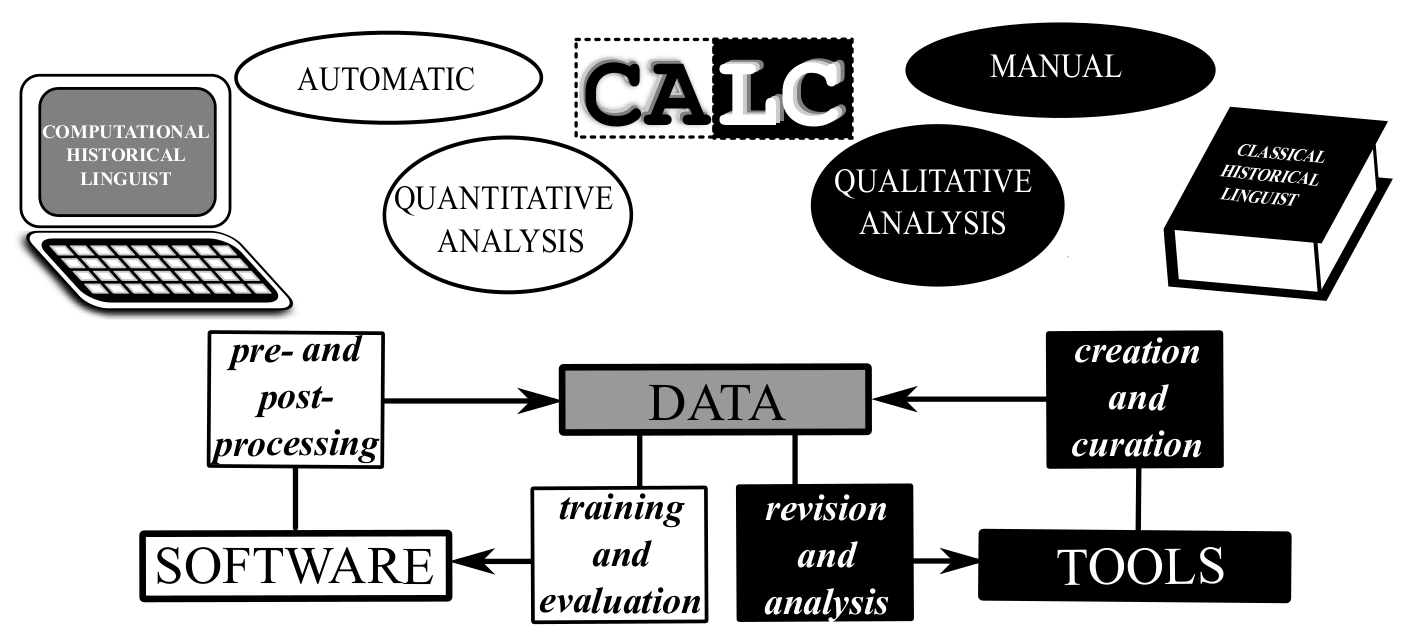
\includegraphics[width=0.75\textwidth]{calc-figure-1.png}
  \caption{Basic idea of data managment within the CALC framework.}
  \label{fig:calc}
\end{figure}

The basic idea behind computer-\emph{assisted} as opposed to computer-\emph{based} language
comparison is to allow scholars to do qualitative and
quantitative research are done at the same time. In order to allow scholars to do this, \textbf{data
must always be available in \emph{machine-} and \emph{human-readable} form}.
Figure \ref{fig:calc} shows a tentative workflow for the CALC framework, in which data is constantly passed back and
forth between computational and classical linguists.

Three different aspects are essential for this workflow:
\begin{itemize}
  \item[(a)] New
software allows for the application of transparent methods which increase the accuracy and the application range
of current methods and also treat the peculiarities of specific language families (like, e.g.,
Sino-Tibetan).
\item[(b)] Interactive tools provide
an interface between human and machine, allowing experts to correct errors and to inspect the automatically
produced results in detail.
\item[(c)] Specific data is used to test and train the software algorithms.
  \end{itemize}



\section{Workflows for Computer-Assisted Language Comparison}

\subsection{Overview}
Our workflows for computer-assisted language comparison have so far been intensively tested on a
small set of 8 Burmish languages, which we investigated in collaboration with Nathan W. Hill, who
was responsible for the qualitative investigation of the data and for the common discussion of new
computer-assisted methods which were then implemented by Johann-Mattis List (see \citealt{Hill2017a}
for an exemplary discussion of some of the new approaches). Our experience with the
Burmish project by now allows us to set up a first workflow that starts from raw data and leads up
to the explicit identification of correspondence patterns across multiple languages. At the moment,
List and Hill develop the workflow further to account also for (semi)-automatic reconstructions, but
in this talk, only the identification of correspondence patterns will be discussed.

\subsection{Details of the Workflow}

Our workflow currently comprises 5 different stages, in which we successively lift linguistic data
from their raw form in which we can find them in wordlists and tables published in dictionaries and
field-work notes, up to a level where correspondence patterns across cognate words have been
automatically identified and can be qualitatively inspected by the scholar.

\begin{figure}[htb]
  \centering
  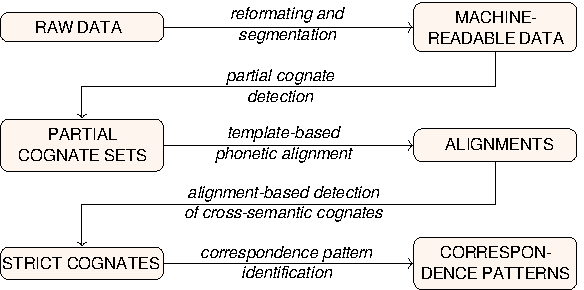
\includegraphics[width=0.8\textwidth]{calc-workflow.pdf}
  \caption{Current state-of-the-art workflow developed in collaboration of different research groups
  working in computer-assisted frameworks.}
  \label{fig:workflow}
\end{figure}

Although the workflow can be carried out almost completely without any manual intervention by a
linguist, we emphasize that this workflow explicitly \emph{allows} for expert intervention at
\emph{any} of the five stages. While, in our experience, specific care is required when lifting the
data the first time to machine-readable format, it should further be noted that \emph{all} steps of
the workflow profit from human intervention, since none of the automatic methods currently available
to us could spot all patterns in linguistic data without over- or underestimating their importance
for linguistic reconstruction.

Our workflow starts from \emph{raw data}, including tabular data from fieldwork notes or data
published in books and articles, which we re-organize and re-format in such a way that the data can
be processed by our tools. Once we have \emph{machine-readable data}, we can use methods for
automatic cognate detection \citep{List2016g} in order to infer \emph{partial cognates} across the
languages in our data. Having inferred cognates, we can now also align the data in the cognate sets.
While we could use phonetic alignment approaches discussed in the literature \citep{List2014d}, we
now use a new approach, based on phonotactic templates, which has the advantage of being much
faster and accurate when dealing with alignments for South-East-Asian languages. Once having
identified the alignments, we start to search automatically for cognates \emph{across} different
concepts. Since all automatic methods \emph{need} to start searching for cognates within the same
concept slot (otherwise, there would be too many false positives), our new method, which makes used
of a systematic comparison of readily aligned cognate sets, systematically searches for cognates
independent of their meaning. The improved, cross-semantic cognate sets, which are all readily
aligned, have the specific property of being \emph{strict}: no cognate set could compare two
morphemes from the same language which would differ in their pronunciation. \citep{List2018PBLOG7}
calls these cognate sets \emph{regular}, but in discussions with Nathan Hill, we decided that
\emph{regular} is probably not the best term, as they can well be wrong, so we call them
\emph{strict} now. Once strict cognates have been identified, we use the new algorithm for the
automatic inference of sound correspondence patterns across multiple languages by \citet{List2019a}
to infer the correspondence patterns in the data.

In Section \ref{sec:wf}, we will provide detailed examples how all steps of the workflow interact,
using a relatively recent collection of linguistic data on Hmong-Mien languages \citep{Chen2012} for
this purpose.
\subsection{Materials and Methods for the Workflow Illustration}

The data we use to illustrate our workflow in the next section was originally collected by
\citet{Chen2012}, and later added in digital form to the Wiktionary project. Chén's collection of
\emph{frequent terms} (\emph{chángyòng cíbiǎo 常用词表}, pp. 567-862) comprises 885 different
concepts translated into 25 varieties of Hmong-Mien. In Figure \ref{fig:data}, we contrast one
exemplary page from Chéns book with the data as it has been prepared by the Wiktionary users.
We can see that the data is essentially the same, but that the rows and columns of the tabular form
have been swapped.

\begin{figure}[htb]
  \centering
  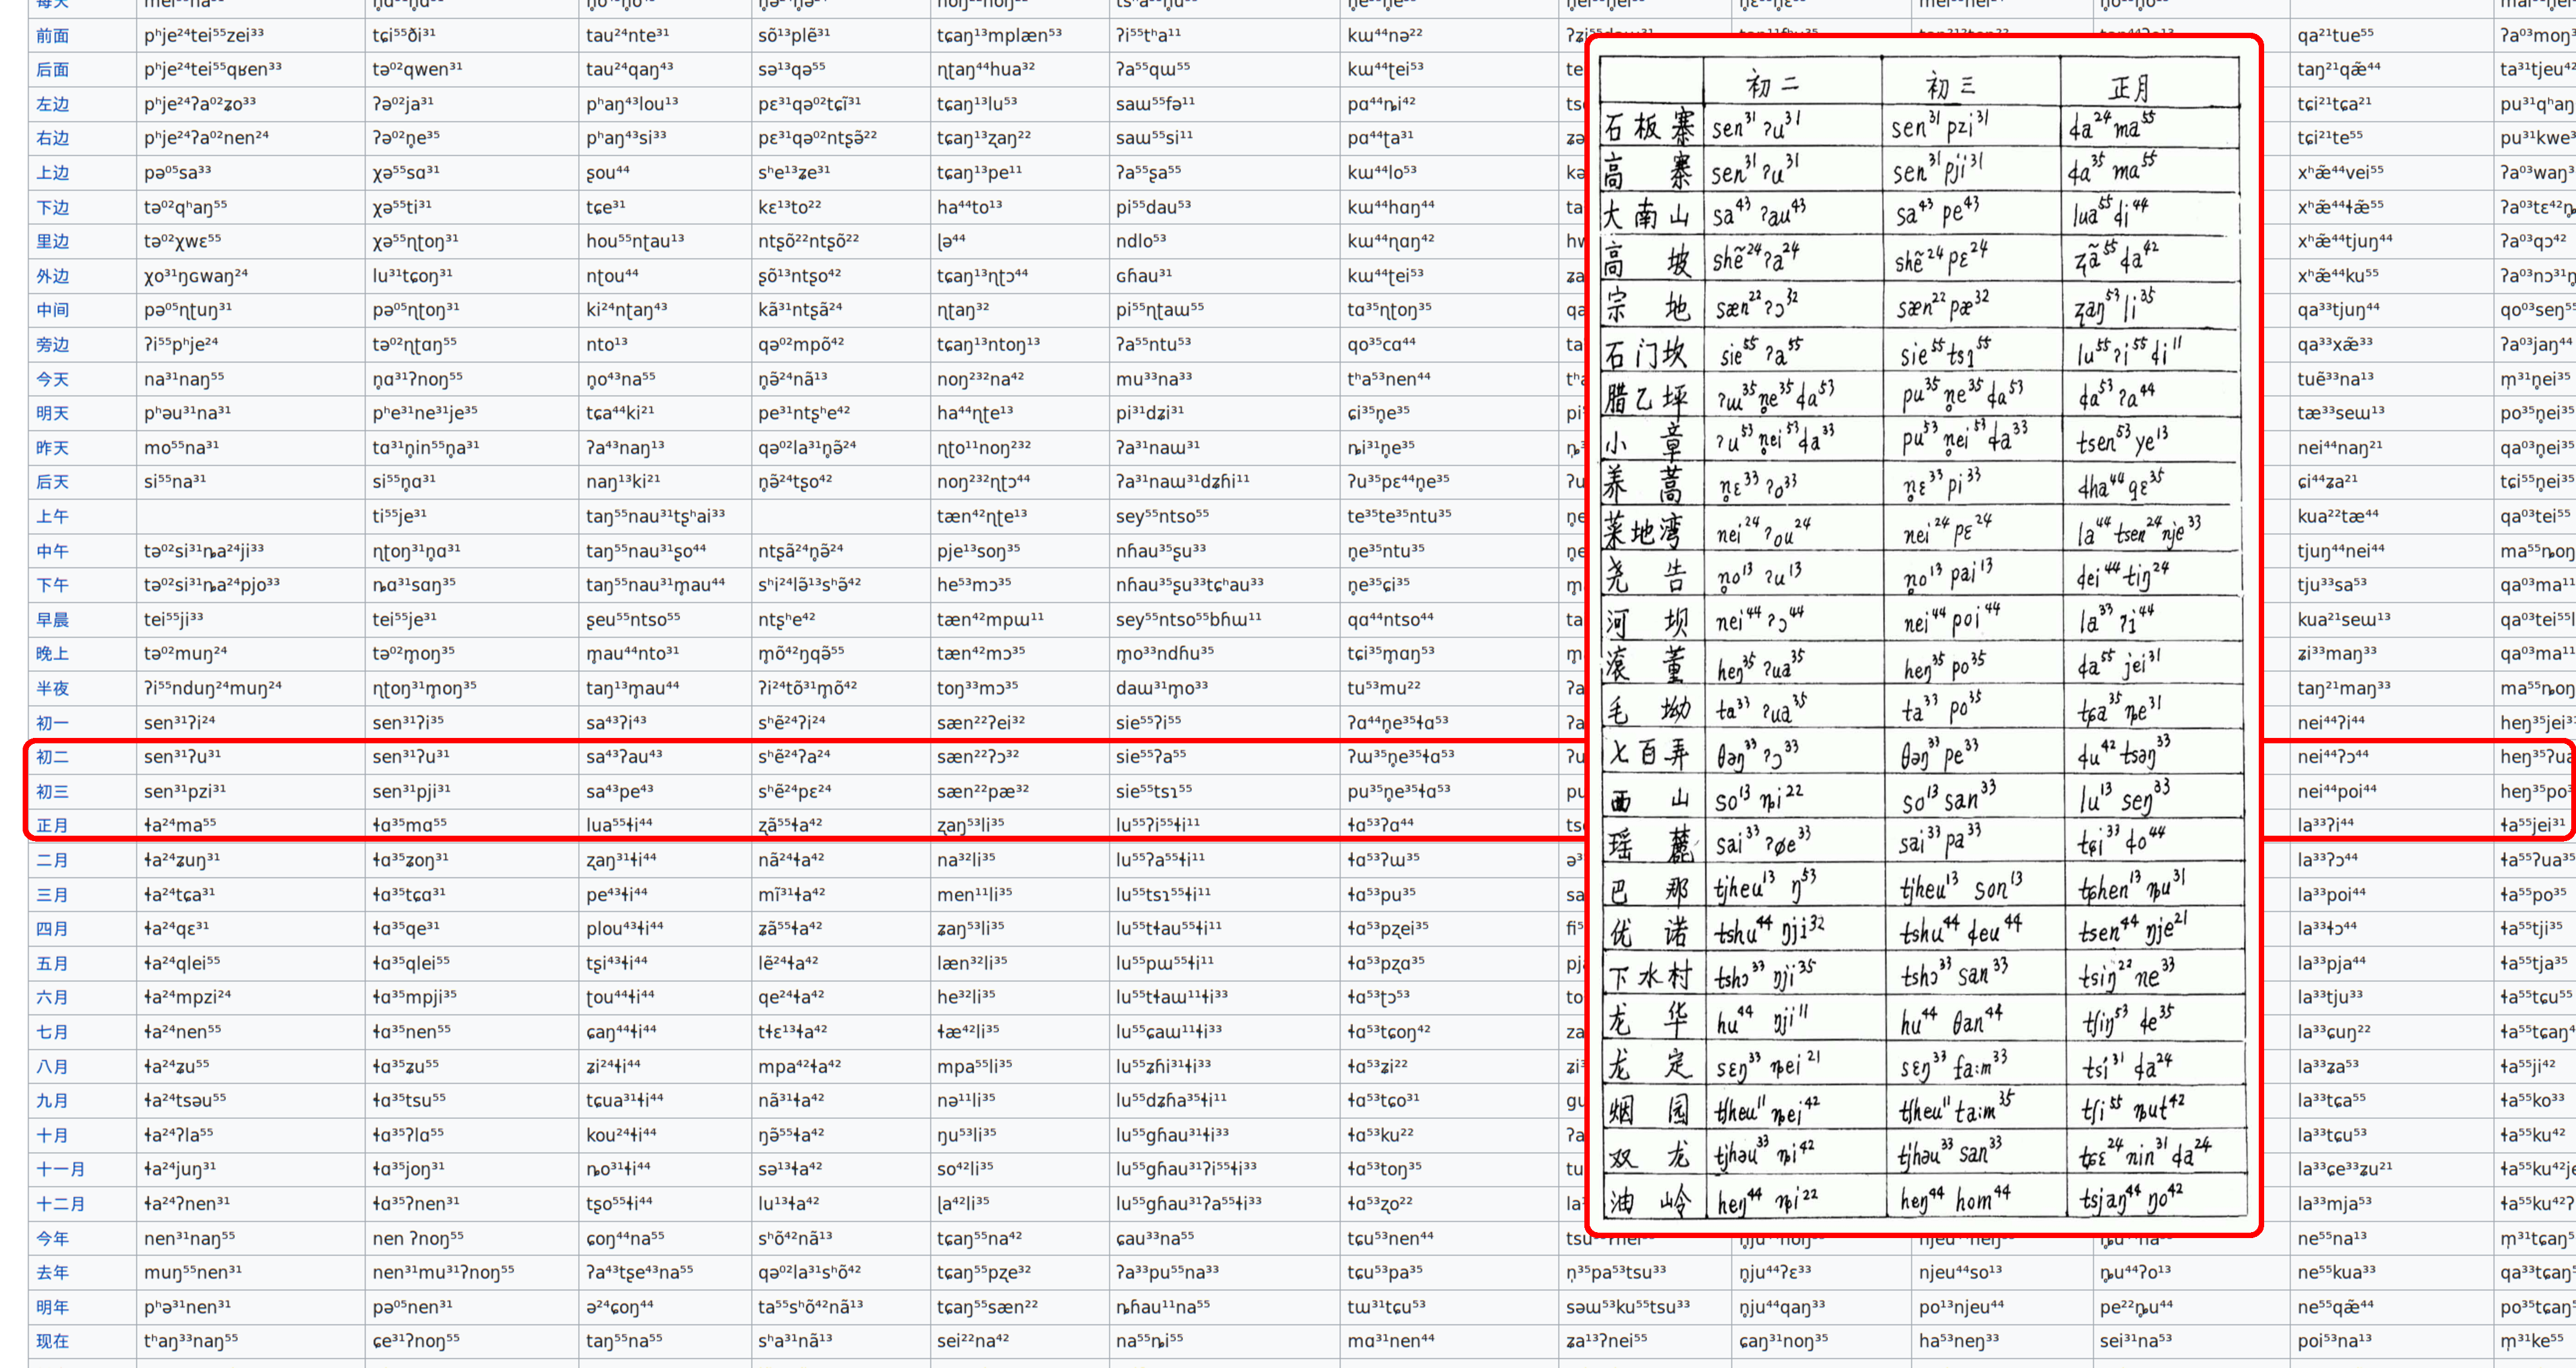
\includegraphics[width=\textwidth]{chen-illustration.pdf}
  \caption{Contrasting Chén's original data with the table in Wiktionary}
  \label{fig:data}
\end{figure}

All methods have either been implemented and published before, or are shared along with the slides
and the handout for this talk. Since this is work in progress, however, we warn users that both data
and code will be in flux for some time, but we will make sure that both data and code can always be
readily analyzed with our tools. All code, the data we use, and installation instructions can be
found at \url{https://github.com/lingpy/calc-workflow}. We ask those interested in testing our
methods to use our issue-tracker on GitHub in case they face difficulties of any kind.
In this talk, we present the workflow with a subset of 10 varieties of Hmong-Mien language. The geographic locations are shown in the figure below.
\begin{figure}[htb]
  \centering
  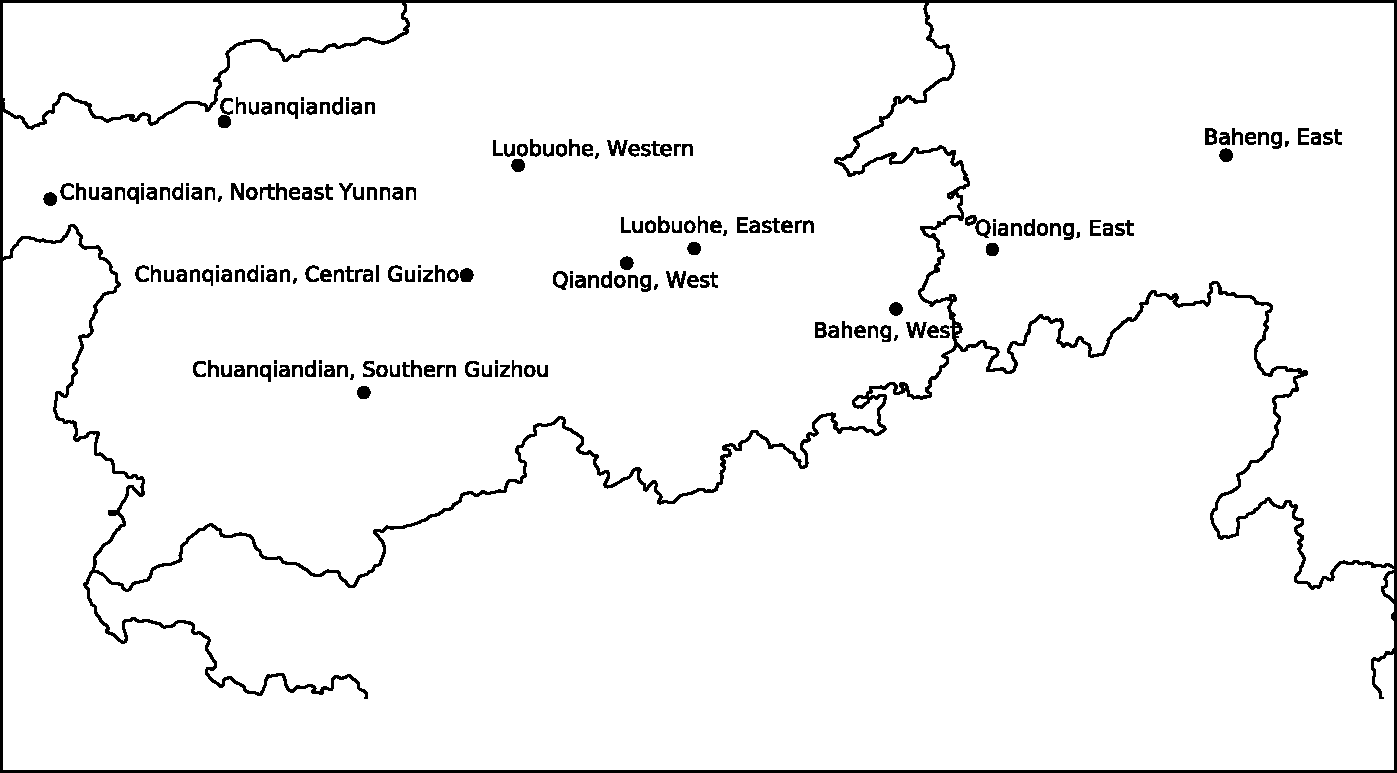
\includegraphics[width=\textwidth]{Geographic.pdf}
  \caption{Language geographic locations}
  \label{fig:geo}
\end{figure}
\section{Illustration of the Workflow}\label{sec:wf}
\subsection{From Raw Data to Segmented Data}
When searching for sound correspondence patterns, we can safely assume that the data is a wordlist; a lexical dataset contains vocabularies which is translated into various languages. The existing wordlists have various presentations, such as, the orientations of data or the usage of seperators of synonyms (\ref{fig:data}). Due to idiosyncratic formats, linguistic datasets often lack interoperability and are therefore not reusable. Following the \textit{Fair} guiding principles of scientific data management from Wilkinson et al., ``Findable, Accessible, Interoperable, and Reusable''\citep{Wilkinson2016}, we convert our raw data into \textit{Lingpy Wordlist} format. 
The format has the following guidelines:

\begin{itemize}
\item A tab-separated input file. 
\item First row serves as a header and defines the content of the rest of the rows. 
\item One value per cell, therefore, synonyms are divided into different rows.
\item Four mandatory columns : unique identification numbers for each row, the language name (DOCULECT), the comparison concept (CONCEPT), the original transcription (International phonetic alphabet, \[IPA\], FORM or VALUE). 
\item TOKENS-columns should supply the supply the transcriptions in space-segmented form.
\end{itemize}

Many existing tools make use of \textit{Lingpy wordlist} format, including the tools we demonstrate here in this talk.

\subsection{From Segmented Data to Cognate Sets}



\textcolor{red}{+++Macy: sentences I am going to use++++The frequency of compound words in South-East Asian (SEA) languages. Partial cognacy.

New algorithm for cognate detection which does not identify cognate words but instead searches for cognate elements in words.}

\begin{itemize}
\item One morpheme correspondent to one cognate id.
\end{itemize}


\subsection{From Cognate Sets to Alignments}

\subsection{From Alignments to Cross-Semantic Cognates}
Words which go back to the same ancestor form can for example have been morphologically modified.
\subsection{From Cross-Semantic Cognates to Sound Correspondence Patterns}

\section{Discussion}

\section{Outlook}




\nocite{List2019a}

\printbibliography
\end{document}
